\section{第二日第四讲}

我们主要研究 $\mathbb F_q$ 上的曲线 $\Sigma$，从我们的观点看它是 2 维算术对象。对 $\mathbb F_q$ 上的曲线 $\Xi$（3 维算术对象），用 $\Sigma\times S^1$ 可得类似的陈述。

在第二日第一讲里，我们描述了如何把 $A_G(\Sigma)$ 变成 $A_G(S^2)$-模（或者按某些人的偏好，变成一个 actegory，即作用范畴）。让我们回顾这个构造。取一点 $x\in\Sigma$，从 $\Sigma\times[0,1]$ 中挖去中心在 $(x,\frac12)$ 的小球。现在可以把它看作从 $\Sigma\sqcup S^2$ 到 $\Sigma$ 的配边。

现在对之作 $A_G$，得到函子 $A_G(S^2)\otimes A_G(\Sigma)\to A_G(\Sigma)$。由于 $A_G(S^2)$ 带有幺半结构（第一日第一讲引入），映射 $A_G(S^2)\otimes A_G(\Sigma)\to A_G(\Sigma)$ 使 $A_G(\Sigma)$ 具有 $A_G(S^2)$-模结构。

当 $\mathcal F_G(\Sigma)=\Bun_G(\Sigma)$ 时有个问题：$\Bun_G$ 是代数几何对象，而 $\Sigma\times[0,1]$ 是拓扑空间，没有代数簇结构。为修补这一点，我们把图中的区间进一步收缩，只在 $\Sigma$ 内留下一个小「泡」（对应此前挖掉的开球）。

\begin{center}
  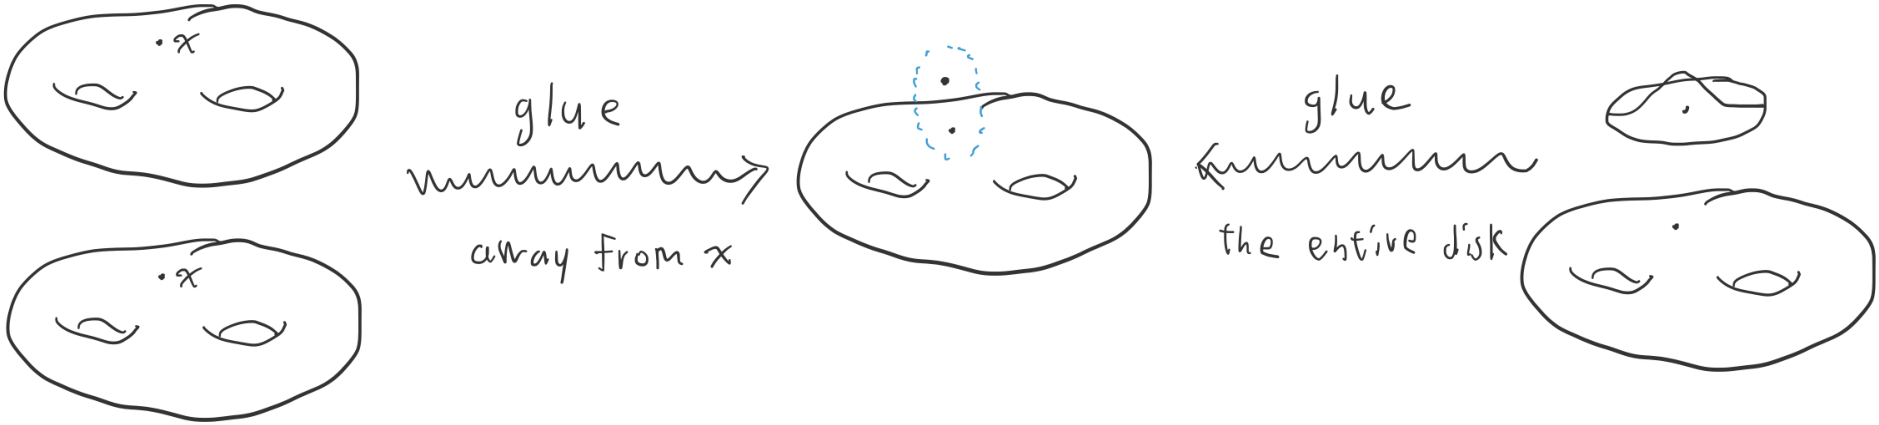
\includegraphics[width=0.92\textwidth]{figures/f71-collapse.png}
\end{center}

更形式地说，这是非分离代数簇「$\Sigma$ 带一个双点」。它可以用下面任一种方式等价描述：
\[
  \Sigma\sqcup_{\Sigma\setminus x}\Sigma=\Sigma\sqcup_D(D\sqcup_{D^\times}D).
\]
这里 $D=\Spec\mathbb F_q[[t]]$ 是形式圆盘，$D^\times=\Spec\mathbb F_q((t))$ 是去心形式圆盘，都以 $x$ 为中心。我们把 $D\sqcup_{D^\times}D$ 称作一个 \textbf{raviolo}，为简单起见记作 $R$。

注意描述 $\Sigma\sqcup_D(D\sqcup_{D^\times}D)$ 现在在代数几何中说得通。我们得到 Hecke 对应
\[
  \begin{array}{ccc}
    & \Bun_G(\Sigma\sqcup_{\Sigma\setminus x}\Sigma=\Sigma\sqcup_D R) & \\[2pt]
    \swarrow & & \searrow \\[2pt]
    \Bun_G(\Sigma)\times\Bun_G(R) & & \Bun_G(\Sigma)
  \end{array}
\]
它由把 $G$-丛限制到簇的相应部分给出。（顶点 $\Bun_G(\Sigma\sqcup_D R)$ 也叫 Hecke 栈。）这是意料之中的：$\Sigma_1$ 与 $\Sigma_2$ 之间的配边应当给出 $\mathcal F_G(\Sigma_1)$ 与 $\mathcal F_G(\Sigma_2)$ 之间的对应。把该对应线性化，得到映射
\[
  A_G(R)\otimes A_G(\Sigma)\to A_G(\Sigma),
\]
也就是说，在 2 维情形这是一个函子；若取 3 维的 $\Xi$ 代替 $\Sigma$，它就是代数同态。回忆 $A_G(\Sigma)=\Shv(\Bun_G(\Sigma))$，其中 $\Shv$ 是某种可构造层范畴：de Rham、Betti 或 étale。

要理解 Langlands，我们首先得理解 $A_G(R)$，它常被称为 Hecke 算子范畴（简称 Hecke 范畴）。为此我们需要几何 Satake 等价。

\begin{rem}
在第一日第一讲中，$A_G(S^2)$ 上有一个幺半结构，它把 $A_G(\Sigma)$ 变成 $A_G(S^2)$-模。用 raviolo 可以同样地操作。现在考虑中心有三个叠置点的 raviolo
\[
  X=D_1\sqcup_{D^\times}D_2\sqcup_{D^\times}D_3.
\]
这是一个（非分离）簇，带有三个自然映射 $p_{12},p_{13},p_{23}$ 到 raviolo $R$（把三个叠置点中任意两个相撞）。定义 $m:A_G(R)\otimes A_G(R)\to A_G(R)$ 为
\[
  m=p_{13,*}(p_{12}^*\otimes p_{23}^*)
\]
（照例，这里的某个 $*$ 可能是 $!$）。当然，我们在此省略了一些细节，因为最后的推前严格说来并不成立（它的定义域是 $A_G(X)$ 而不是 $A_G(X)\otimes A_G(X)$）。

与真正的 $S^2$ 的情形类似，可以证明 $A_G(R)$ 是一个 $E_3$-范畴（这里有一些代数几何的技术细节）。特别地，$A_G(R)$ 是对称幺半范畴。

也可以给图景加上分歧。作用是一样的：在中间切一个球。无分歧点处的代数/范畴也一样。然而在分歧点 $x_0\in\Sigma$ 处，球无法离开区间 $x_0\times[0,1]$，于是我们没有 $E_3$-结构。
\end{rem}

我们再引入一些记号：记 $F=\mathbb F_q((t))$，$O=\mathbb F_q[[t]]$ 为 $F$ 的整数环。

我们用双陪集来描述 $A_G(R)=\Shv(\Bun_G(R))$。回忆 $R=D_1\sqcup_{D^\times}D_2$。$R$ 上一个 $G$-丛（同构意义下）由以下数据给出：每个 $D_i$ 上的一个 $G$-丛，加上一个粘接函数 $g:D^\times=D_1\cap D_2\to G$。$D_i$ 上的丛总是平凡的，而粘接函数按定义就是 $G(F)$ 中的元素。此外，两个粘接函数 $g,g'$ 定义同构的 $G$-丛，当且仅当 $g'=h_1gh_2^{-1}$ 对某个 $h_1,h_2\in G(O)$ 成立。因此我们刚刚证明了

\begin{lem}
  $\Bun_G(R)=G(O)\backslash G(F)/G(O)$。
\end{lem}

\begin{rem}
设 $G$ 半单。利用一个（更难的）事实：射影的 $\Sigma$ 上任何主 $G$-丛都在某点之外平凡化（这归功于 Harder），可以把论证搬到一般的 $\Bun_G(\Sigma)$ 上。这与本讲无关。
\end{rem}

注意 $G(F)/G(O)=LG/L^+G=\Gr$ 按定义就是 $G$ 的仿射 Grassmann 流形。于是 $\Bun_G(R)=G(O)\backslash\Gr=\Gr$ 是 $G$ 的「$G(O)$-等变仿射 Grassmann 流形」。因此 Hecke 范畴 $A_G(R)$ 是
\[
  H=\Shv(\Gr)=\Shv_{G(O)}(\Gr),
\]
即仿射 Grassmann 流形上 $G(O)$-等变可构造层的（导出）范畴。在 3 维情形，我们将得到 Hecke 代数 $H=\Fun(\Gr(\mathbb F_q))$。

在第二日第二讲里我们讨论了经典 Satake 同构：
\[
  \Fun(\Gr/\mathbb F_q)\cong K_0(\Rep\check G)\cong O(\check G/\check G)=O(\Maps(S^1,*/\check G)).
\]
现在我们把该同构范畴化，先得到几何 Satake 等价，再得到导出几何 Satake 等价。

考虑仿射 Grassmann 流形上 $G(O)$-等变反常层（perverse sheaves）的 Abel 范畴，记作 $\Shv(\Gr)^\heartsuit$。同样地，可以用任何层论：étale、Betti 或 de Rham。文献中也用记号 $\mathrm{Perv}(\Gr)$。（事实上按定义，$\mathrm{Perv}(\Gr)$ 就是 $G(O)$-等变可构造层导出范畴 $\Shv(\Gr)$ 上 $t$-结构的核心。）

\begin{thm}[几何 Satake 等价]
存在对称幺半范畴的等价
\[
  \Shv(\Gr)^\heartsuit\cong\Rep(\check G),
\]
其中 $\Shv(\Gr)^\heartsuit$（相应地 $\Rep(\check G)$）上的幺半结构是反常层的卷积（相应地表示的张量积）。
\end{thm}

\begin{rem}
  \begin{enumerate}[label=(\arabic*),leftmargin=1.8em,itemsep=0.2em]
    \item 注意两个范畴都带有到向量空间的自然函子：遗忘函子
    \[
      \Rep(\check G)\to\Vect,
    \]
    与上同调函子
    \[
      H^*_{G(O)}(\Gr,-):\ \Shv(\Gr)^\heartsuit\to\Vect
    \]
    （用 $t$-结构定义）。它们称为纤维函子，而几何 Satake 等价与这两个函子相容。但若用 $\mathrm{GrVect}$（分次向量空间）代替 $\Vect$，则需要 Koszul 符号法则。
    \item 把该等价取到 Grothendieck 环 $K_0$ 的层面（或取恒等函子的迹），就恢复出经典 Satake 同构。
    \item 作为对称幺半范畴的等价，它特别地意味着 $\Shv(\Gr)^\heartsuit$ 上的幺半结构是交换的。下面是直接的说明。我们已看到 $\Shv(\Gr)^\heartsuit$ 是 $E_3$-范畴。范畴上的 $E_n$-结构由以 $\mathbb R^n$ 中点的构型空间为标号的一族乘法组成。随着 $n$ 增大，这些乘法变得越来越交换。$n=1$ 时得到幺半范畴；$n=2$ 时得到辫幺半范畴（即 $a\otimes b$ 同构于 $b\otimes a$，但这些同构不必是对合的）；最后当 $n=3$ 时，第一个乘法必然变成交换的，于是得到对称幺半范畴。
  \end{enumerate}
\end{rem}

由几何 Satake 等价，对任意点 $x\in\Sigma$，我们有 $\Shv(\Gr)^\heartsuit\cong\Rep\check G$ 在 $A_G(\Sigma)=\Shv(\Bun_G(\Sigma))$ 上的（受限）Hecke 作用。由于 $x\in\Sigma$ 的选取是任意的，为更典范起见，我们得把所有点都算进去。为此可以引入 $\Rep(\check G)$ 的阿代尔版本：受限张量积
\[
  \bigotimes_{x\in\Sigma}{}^{\mathrm{restr}}\,\Rep\check G.
\]
上述作用一般而言是神秘的，人们希望把它「对角化」。为此我们求助于
\[
  \bigotimes_{x\in\Sigma}{}^{\mathrm{restr}}\,\Rep\check G\ \ \text{在}\ \ \QCoh(\Loc_{\check G}\Sigma)\ \ \text{上的作用}.
\]
再说一次，任何版本的局部系（de Rham、Betti、étale）都完全适用。

\textbf{约定}：至少在本讲中，我们把谱理论（即下文所说的朴素 B-理论）的系数域取为 $\mathbb C$。

为更精确地描述该作用，先固定某个 $x\in\Sigma$。有等同
\[
  \Loc_{\check G}\Sigma=\Maps(\Sigma,*/\check G)
\]
（局部常值映射）。然后定义 $\mathrm{ev}_x:\Loc_{\check G}\Sigma\to*/\check G$ 为在 $x$ 处取值。（等价地，可以把任意 $\check G$-局部系限制到点 $x\in\Sigma$，这给出映射 $\Loc_{\check G}\Sigma\to*/\check G$。）另一方面，每个表示都定义了点上（更精确地说，$*/\check G$ 上）的一个向量丛，于是有等同
\[
  \QCoh(*/\check G)=\Vect(*/\check G)=\Rep\check G.
\]
因此给定任意表示 $V\in\Rep(\check G)$，可沿 $\mathrm{ev}_x$ 拉回，得到 $\Loc_{\check G}\Sigma$ 上的拟凝聚层 $\mathrm{ev}_x^*V$；而 $V$ 在 $\QCoh(\Loc_{\check G}\Sigma)$ 上的作用就是与 $\mathrm{ev}_x^*V$ 作张量积。这延拓为 $\bigotimes\nolimits_{x\in\Sigma}^{\mathrm{restr}}\Rep\check G$ 的真正作用。

\begin{rem}
若 $\Sigma$ 定义在 $\mathbb F_q$ 上，则对任意 $x\in\Sigma(\mathbb F_q)$ 还可以联系一个映射 $\Loc_{\check G}\Sigma\to\check G/\check G$。这是因为 Frobenius 态射扮演了 $S^1$ 的角色。
\end{rem}

天真地，人们可以把几何 Langlands 对应表述为：作为 $\bigotimes\nolimits_{x\in\Sigma}^{\mathrm{restr}}\Rep\check G$-模，$\Shv(\Bun_G(\Sigma))$ 与 $\QCoh(\Loc_{\check G}\Sigma)$ 是否等价？
答案是否定的。关键原因是：$\bigotimes\nolimits_{x\in\Sigma}^{\mathrm{restr}}\Rep\check G$ 在 $\QCoh(\Loc_{\check G}\Sigma)$ 上的作用是局部常值的，而在 $\Shv(\Bun_G(\Sigma))$ 上的作用完全不是局部常值的。

为了有等价，我们要么把右端换成 $\IndCoh(\Loc_{\check G}\Sigma)$（ind-凝聚层），要么把左端换成 tempered 层。

\begin{rem}
对每种层论（de Rham、Betti 与 étale），都有一个谱作用定理，它们大致都可以概括为下面这条。
\end{rem}

\begin{thm}[谱作用]
$\bigotimes\nolimits_{x\in\Sigma}^{\mathrm{restr}}\Rep\check G$ 在 $A_G(\Sigma)=\Shv(\Bun_G(\Sigma))$ 上的作用经过 $\QCoh(\Loc_{\check G}\Sigma)$-作用分解。
\end{thm}

尽管如此，让我们（暂时）朴素地研究 $\QCoh(\Loc_{\check G}\Sigma)$。于是我们考虑 B-理论：它给 2 维流形 $\Sigma$ 配 $B_{\check G}(\Sigma)=\QCoh(\Loc_{\check G}\Sigma)$，给 3 维流形 $\Xi$ 配向量空间 $B_{\check G}(\Xi)=O(\Loc_{\check G}\Xi)$。与 A-理论不同，这定义了真正的 TQFT：输出只依赖 $\Sigma$ 或 $\Xi$ 的拓扑。

与 A-理论一样，我们得先花点时间看 $B_{\check G}(R)$。由于 raviolo 不过是一个带双点的圆盘，可以把 $R$ 上的局部系等同于圆盘 $D^2$ 上的一对局部系，连同它们在 $S^1=\partial D^2$ 上的一个等同。于是可以算出
\[
  \Loc_{\check G}(R)=\Loc_{\check G}(D^2)\times_{\Loc_{\check G}(S^1)}\Loc_{\check G}(D^2).
\]
若暂时取 Betti 作为层论，则得到（栈的）等同
\[
  \Loc_{\check G}(D^2)=\{\pi_1(D^2)\to\check G\}/\check G=*/\check G,\qquad
  \Loc_{\check G}(S^1)=\{\pi_1(S^1)\to\check G\}/\check G=\check G/\check G
\]
（两处 $\check G$ 都按共轭作用）。它们给出等同
\[
  \Loc_{\check G}(R)=*/\check G\times_{\check G/\check G}*/\check G=(*\times_{\check G}*)/\check G.
\]
这里点 $*$ 作为单位元映入 $\check G$。因此取纤维积 $*\times_{\check G}*$ 时只用到单位元的邻域。由此可见可以把 $\check G$ 换成它的 Lie 代数 $\check{\mathfrak g}$，得到等同
\[
  *\times_{\check G}*=*\times_{\check{\mathfrak g}}*=\Omega\check{\mathfrak g},
\]
其中 $\Omega\check{\mathfrak g}$ 是 $\check{\mathfrak g}$ 的环路空间。

对一般的向量空间 $V$，$*\times_V*$ 是点 $*$ 的自交。对通常的代数簇，我们会算
\[
  *\times_V*=\Spec\mathbb C\times_{\Spec\Sym V^*}\Spec\mathbb C=\Spec(\mathbb C\otimes_{\Sym V^*}\mathbb C).
\]
但我们工作在导出情形，这意味着最后一步应取导出张量积。写出 Koszul 复形即可看出，$\mathbb C\otimes^L_{\Sym V^*}\mathbb C$ 是 $\dim V$ 个次数为 $1$ 的变量的外代数。可以验证两侧的乘法相同，且有自然同构
\[
  \mathbb C\otimes^L_{\Sym V^*}\mathbb C=\Sym V^*[1].
\]
这里 $1$ 是上同调移位，特别地 $\Sym V^*[1]$ 是外代数。

于是近似地，$B_{\check G}(R)$ 就是 $\QCoh(\Loc_{\check G}(R))=\Sym\check{\mathfrak g}^*[1]\text{-}\mathrm{Mod}_{\check G}$。注意幺半结构不是模的张量积，而是由
\[
  \Loc_{\check G}(R)=*/\check G\times_{\check G/\check G}*/\check G
\]
是同一栈的两份拷贝的纤维积这一事实而来的卷积。这一点可以用幺半结构的「裤子」（pair of pants）定义验证。

\begin{rem}[Koszul 对偶]
给定带增广 $\epsilon:\Lambda\to k$ 的外 $k$-代数 $\Lambda$，考虑函子 $\Hom_\Lambda(k,-):\Lambda\text{-}\mathrm{Mod}\to\End_\Lambda(k)\text{-}\mathrm{Mod}$。其中
\begin{enumerate}[label=(\arabic*),leftmargin=1.8em,itemsep=0.2em]
  \item $\Lambda\text{-}\mathrm{Mod}$ 上的幺半结构由卷积给出：给定两个 $\Lambda$-模，沿 $\epsilon$ 把它们推到 $k$-模，取张量积，再沿 $\epsilon$ 拉回；
  \item $\End_\Lambda(k)$ 对 $\Hom_\Lambda(k,M)$ 的作用由与自同态作前复合给出。
\end{enumerate}
除非仔细规定所考虑的模的类别，这个函子并不是模的导出范畴的等价。事实上，它限制为凝聚 $\Lambda$-模与完美 $\End_\Lambda(k)$-模之间的等价。

上面的 Koszul 对偶可以提升到局部算子范畴，建立等价
\[
  \Coh(\Loc_{\check G}(R))\cong\Perf(\check{\mathfrak g}^*[2]/\check G).
\]
把这两个范畴作 ind-完备化，又得到
\[
  \IndCoh(\Loc_{\check G}(R))\cong\QCoh(\check{\mathfrak g}^*[2]/\check G)
\]
之间的等价。这是幺半范畴的等价：右端带有通常的幺半结构，而左端相应的幺半结构是从 $\Omega\check{\mathfrak g}$ 的群胚结构而来的卷积。
\end{rem}

回到 A-与 B-理论，我们准备陈述几何 Satake 等价的导出版本（不带核心的那一个）。我们天真地要求 $A_G(R)=\Shv(\Gr)$ 与 $B_{\check G}(R)=\QCoh(\Loc_{\check G}R)$ 之间的等价。正如已经说过的，这并不正确，正确版本如下。

\begin{thm}[导出几何 Satake 等价]
存在对称幺半范畴的等价
\[
  \Shv(\Gr)\cong\IndCoh(\Omega\check{\mathfrak g}/\check G)=\QCoh(\check{\mathfrak g}^*[2]/\check G).
\]
\end{thm}

\begin{rem}
\begin{enumerate}[label=(\arabic*),leftmargin=1.8em,itemsep=0.2em]
  \item 提请注意：导出几何 Satake 等价的右端出现了余伴随表示，这是诸多迹象之一，说明矩映射（进而 Hamilton 作用）将在我们的故事中起作用。这将在此后各讲中成为一个大主题。
  \item 与几何 Satake 等价的情形类似，导出几何 Satake 等价中的范畴也带有纤维函子。在仿射 Grassmann 流形一侧，可以取等变上同调
  \[
    H^*_{G(O)}(\Gr,-):\ \Shv(\Gr)\to H^*_{G(O)}(\mathrm{pt})\text{-}\mathrm{Mod}.
  \]
  另一侧有函子
  \[
    \QCoh(\check{\mathfrak g}^*[2]/\check G)\to O(\check{\mathfrak g}^*[2]/\check G)\text{-}\mathrm{Mod},
  \]
  由限制到 Kostant 切片给出（这里不作解释）。由若干计算可知
  \[
    \begin{aligned}
      O(\check{\mathfrak g}^*[2]/\check G)&=O(\check{\mathfrak g}^*[2])^{\check G}=\Sym\check{\mathfrak t}[2]^W=\Sym\mathfrak t^*[2]^W\\
      &=\Sym\mathfrak t[-2]^W=\Sym\mathfrak g[-2]^G=H^*_{G(O)}(\mathrm{pt}).
    \end{aligned}
  \]
  同样地，该等价与这两个纤维函子相容。
\end{enumerate}
\end{rem}
